\documentclass[11pt]{article}
\usepackage{lmodern,setspace,amsmath,amssymb,amsfonts,amsthm,graphicx,multicol,grffile,float}
\usepackage{authblk,url,csvsimple,cuted,dblfloatfix,parskip}
\usepackage[a4paper, top=0.9in, bottom=1.05in, left=1.01in, right=1.01in]{geometry}
\usepackage[polish]{babel}
\usepackage[utf8]{inputenc}
\usepackage[unicode]{hyperref}
\usepackage{listings}
\usepackage{booktabs}
\title{Informatyka w Medycynie - Projekt 1\\ Tomograf komputerowy}
\author{Dariusz Max Adamski 136674, Sławomir Gilewski 142192}
\affil{\{dariusz.adamski,slawomir.gilewski\}@student.put.poznan.pl}
\date{Data oddania: \today}

\def\code#1{\texttt{#1}}

\begin{document}

\maketitle

\section*{Wstęp}

W danym sprawozdaniu przedstawiony będzie symulator tomografu komputerowego, z wykorzystaniem transformaty radona. Następnie wygenerowany zostaje obraz wyjściowy, wykonując odwrotną transformatę na uzyskanym wcześniej sinogramie. 

\begin{figure}[h!]
	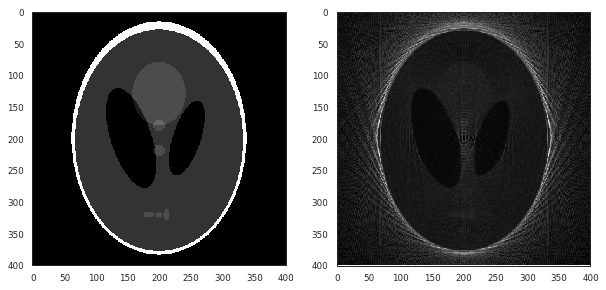
\includegraphics[width=\linewidth]{res/demo.png}
	\caption{Przykład działania programu}
	\label{fig:demo}
\end{figure}


\section{Model tomografu}

Zastosowany przez nas model tomografu to model równoległy. Zdecydowaliśmy się na to rozwiązanie, ponieważ było wygodne w implementacji. Po wyznaczaniu współrzędnych punktów odpowiadających emiterowom, wyznaczenie współrzędnych odpowiadających detektorom przebiega analogicznie.

\section{Narzędzia}

\subsection{Język Programowania}
Wybraliśmy język programowania Python. Głównie ze względu na jego prostotę i łatwość instalowania i korzystania z dodatkowych bibliotek. Jest to język, w którym obydwoje najbardziej swobodnie się poruszamy.

\subsection{Dodatkowe biblioteki}
Istotne biblioteki i ich wykorzystanie w naszym programie to:
\begin{itemize}
    \item Numpy: Obliczenia i operacje na n-wymiarowych macierzach
    \item Pydicom: Wykorzystana przy zapisie i odczycie obrazów w standardzie DICOM
    \item Skimage:  Wszelkiego rodzaju odczyt, operacje i przekształcenia na obrazach
    \item Scipy: Funkcje związane z transformatami Fouriera, wykorzystanymi przy filtrowaniu sinogramu w celu redukcji szumu
    \item Matplotlib: Wszelkiego rodzaju wizualizacje
    \item Multiprocessing: Urównolegnienie transformaty Radona, w celu jej przyspieszenia
\end{itemize}

\section{Funkcje programu}

Opis głównych funkcji programu oraz ilustracja za pomocą fragmentów kodu źródłowego

\subsection{pozyskiwanie odczytów dla poszczególnych detektorów}
\begin{verbatim}
def single_radon_transform(detector_count, angle_range, image, radius, center, alpha):
    emitters = emitter_coords(alpha, angle_range, detector_count, radius, center)
    detectors = detector_coords(alpha, angle_range, detector_count, radius, center)
    lines = radon_lines(emitters, detectors)
    result = rescale(np.array([np.sum( image[tuple(line)]) for line in lines]))
    return result
\end{verbatim}
Dla konkretnego kroku alpha:
\begin{enumerate}
  \item emiter\_coords, detector\_coords: Pozyskujemy współrzędne emiterów oraz detektorów dla wybranych parametrów(ilość emiterów/detektrów, rozpiętość układu) oraz wybranego obrazu (potrzebujemy promień oraz współrzędne środka)
  \item radon\_lines: Dla uzyskanych współrzędnych emiterów oraz detektorów obliczamy współrzędne wszystkich pixeli leżących na prostych pomiędzy tymi punktami. Wykorzystujemy algorytm Bresenhama do liniowego przejścia po kolejnych pikselach obrazu dyskretnego.
  \item Następnie dla pozyskanych wcześniej współrzędnych pikseli, sumujemy ich wartości dla każdej pary emiter/detektor.
\end{enumerate}
W celu uzyskania całego sinogramu, iterujemy po kolejnych wartościach alfy, wykorzystując powyższy algorytm w funkcji ,,radon\_transform''. Warto wspomnieć iż algorytm pracuje na zmodyfikowanym obrazie wejściowym - przed zastosowaniem transformaty, do obrazu dodawany jest padding, aby zapobiec utracie informacji.

\subsection{Filtrowanie sinogramu}
W celu uzyskania lepszych wartości wynikowych, przed przystąpieniem do odwrotnej transformaty radona zostaje zastosowany splot na naszym sinogramie.
\begin{verbatim}
def filter_sinogram(sinogram):
    n = sinogram.shape[0]
    filter = 2 * np.abs(
    fftfreq(n).reshape(-1, 1))
    result = ifft(fft(sinogram, axis=0) * filter, axis=0)
    result = clip(np.real(result), 0, 1)
    return result
\end{verbatim}
\begin{figure}[h!]
	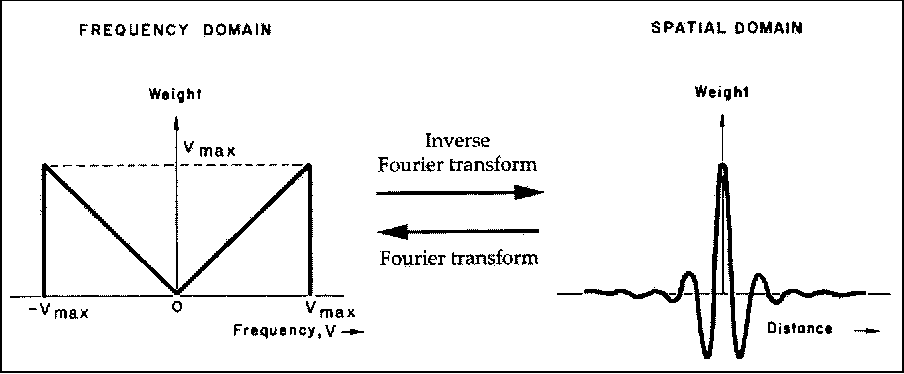
\includegraphics[width=\linewidth]{res/ramp_filter.png}
	\caption{Po lewej stronie ,,ramp filter'' w dziedzinie częstotliwości, a po prawej w dziedzinie przestrzennej}
\end{figure}
\begin{enumerate}
    \item Najpierw tworzymy nasz kernel/filtr w dziedzinie częstotliwości (frequency domain). Po przeprowadzonych eksperymentach, doszliśmy do wniosku, że najlepiej wypada tutaj ,,ramp filter''.
    \item Następnie przekształcamy nasz sinogram do dziedziny częstotliwości za pomocą funkcji fft.
    \item Przekształcony sinogram przemnażamy przez stworzony wcześniej filtr.
    \item Wynikowy sinogram przekształcamy z powrotem do dziedziny przestrzennej (spatial domain). Ucinane są również wartości poniżej 0 oraz powyżej 1 w sinogramie.
Uznaliśmy, iż rozmiar maski najlepiej pozostawić taki, jak rozmiar sinogramu, czyli ilość detektorów transformaty.
\end{enumerate}

\subsection{Ustalanie jasności poszczególnych punktów obrazu wynikowego oraz jego przetwarzanie końcowe}
\begin{verbatim}
    def single_inverse_radon_transform(image, tmp, single_alpha_sinogram, alpha,
    detector_count, angle_range, radius, center):
        emitters = emitter_coords(alpha, angle_range, detector_count, radius, center)
        detectors = detector_coords(alpha, angle_range, detector_count, radius, center)
        lines = radon_lines(emitters, detectors)
        for i, line in enumerate(lines):
            image[tuple(line)] += single_alpha_sinogram[i]
            tmp[tuple(line)] += 1
\end{verbatim}
\begin{enumerate}
\item Początek funkcji przebiega analogicznie do wcześniej omówionej transformaty radona. Dla konkretnego kroku alpha: pozyskujemy współrzędne emiterów oraz detektorów a następnie dla uzyskanych punktów obliczamy współrzędne wszystkich pixeli leżących na prostych pomiędzy tymi nimi.
\item Następnie dla każdej pary emiter/detektor, dodajemy wartość odpowiadającego punktu sinogramu do pikseli leżących na linii pomiędzy nimi.
\item W macierzy tmp dla każdego pixela przechowywana jest liczba linii, które przez niego przeszły. Macierz ta wykorzystana jest później w celu normalizacji obrazu wynikowego.
\end{enumerate}
W celu uzyskania całego obrazu wynikowego, iterujemy po kolejnych wartościach alfy, wykorzystując powyższy algorytm w funkcji ,,inverse\_radon''. \\
Po przejściu przez wszystkie wartości alpha, funkcja ta wykorzystuje wspomnianą wcześniej macierz tmp w celu normalizacji obrazu. \\
Na koniec wycinany jest obraz wynikowy, w celu odrzucenia dodanego wcześniej paddingu.






\subsection{Wyznaczanie wartości miary RMSE na podstawie obrazu źródłowego oraz wynikowego}

Przeprowadziliśmy eksperyment sprawdzający wpływ poszczególnych parametrów transformaty na jakość odtworzonego obrazu. Jako miary użyliśmy błędu średniokwadratowego (RMSE). Zgodnie z poleceniem ,jakop parametry domyślne przyjęliśmy 180 detektorów, 180 skanów oraz rozpiętość wachlarza równą 180. Jeśli nie powiedziano inaczej, do testów użyliśmy obrazu ,,saddle-pe'', widoczny na rysunku \ref{fig:filter-2}.

Na rysunku \ref{fig:rmse} przedstawiony jest błąd przy zmieniającej się odpowiednio liczbie skanów, detektorów i rozwartości kątowej (wynikowe obrazki widoczne na rysunkach na ostatniej stronie). Według nas zwiększanie każdego z parametrów zwiększa jakość obrazu, przy czym większa liczba skanów i detektorów redukuje szum/ziarnistosć obrazu. Jednak na wykresach RMSE niestety nie widać znaczących zmian. Według nas jest to spowodowane dużą ilością szumu w obrazach wyjściowych.

Dodatkowo sprawdziliśmy wpływ filtrowania sinogramu na jakość obrazu. Wyniki są przedstawione na rysunkach \ref{fig:filter-1} i \ref{fig:filter-2}, oraz w tabeli \ref{tab:filter}.
Według nas filtrowanie zdecydowanie poprawia odzwierciedlenie obrazu, w szczególności jasność elementów na obrazie jest bardziej zbliżona do oryginału. Zredukowana jest też okrągła poświata.
Filtrowanie na obrazie ,,shepp-logan'' zdecydowanie zredukowało błąd, ale przy ,,saddle-pe'' niestety już nie (jednak według nas obraz jest odrobinę ostrzejszy).

\begin{figure}[h]
	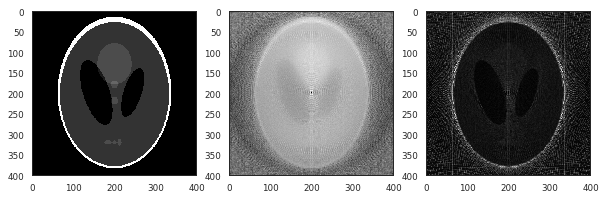
\includegraphics[width=\linewidth]{res/filter1.png}
	\caption{Wizualizacja efektów filtrowania sinogramu (shepp-logan). Po lewej stronie oryginalny obrazek, na środku efekt odwrotnej transformaty Radona bez filtrowania, a po prawej z filtrowaniem}
	\label{fig:filter-1}
\end{figure}

\begin{figure}[h]
	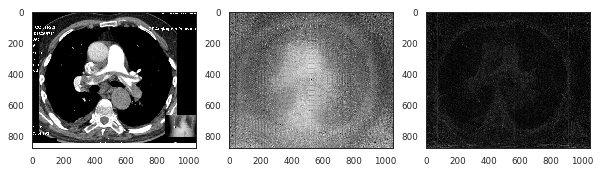
\includegraphics[width=\linewidth]{res/filter2.png}
	\caption{Wizualizacja efektów filtrowania sinogramu (saddle-pe)}
	\label{fig:filter-2}
\end{figure}

\begin{figure}[h]
	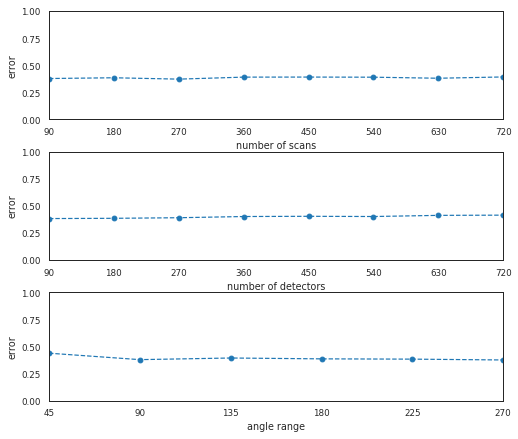
\includegraphics[width=\linewidth]{res/rmse.png}
	\caption{Wartość RMSE przy zmienającej się liczbie skanów, detektorów i rozwartości kątowej}
	\label{fig:rmse}
\end{figure}

\begin{table}
    \centering
    \caption{Wyniki eksperymentu}
    \label{tab:filter}
    \begin{tabular}{llll}
    \toprule
    obrazek     & rysunek & RMSE (bez filtrowania) & RMSE (z filtrowaniem) \\
    \midrule
    shepp-logan & rysunek \ref{fig:filter-1} & 0.482961 & 0.195934 ($\downarrow$) \\
    saddle-pe   & rysunek \ref{fig:filter-2} & 0.365851 & 0.371541 ($\uparrow$) \\
    \bottomrule
    \end{tabular}
\end{table}

\newpage

\subsection{Obsługa plików DICOM}

Do obsługi plików DICOM wykorzystaliśmy bibliotekę \code{pydicom}.

W naszym programie odczyt jest realizowany przez funkcję \code{read\_dicom}, która przyjmuje ścieżkę do pliku który chcemy otworzyć i zwraca obraz w postaci 2-wymiarowej macierzy oraz słownik metadanych, które zawierają na przykład imię pacjenta.

\begin{verbatim}
image, meta = read_dicom('test.dcm')
\end{verbatim}

Pliki DICOM zapisujemy przy użyciu funkcji \code{write\_dicom}, która przyjmuje ścieżkę pod którą będzie zapisany plik, obrazek w formie 2-wymiarowej macierzy oraz słownik metadanych.
Gdy nie podamy żadnych metadanych, w pliku zostaną umieszczone tylko te, aby plik był zgodny ze standardem DICOM.

\begin{verbatim}
write_dicom('test.dcm', image, dict(
    PatientName='Doe^John',
    PatientID='666',
    ImageComments='No comment :)',
    StudyDate='20200213',
))
\end{verbatim}

Poprawność zapisu plików DICOM zweryfikowaliśmy przy pomocy przeglądarki 
\url{https://www.imaios.com/en/Imaios-Dicom-Viewer}.


\newpage

\begin{figure}[h]
	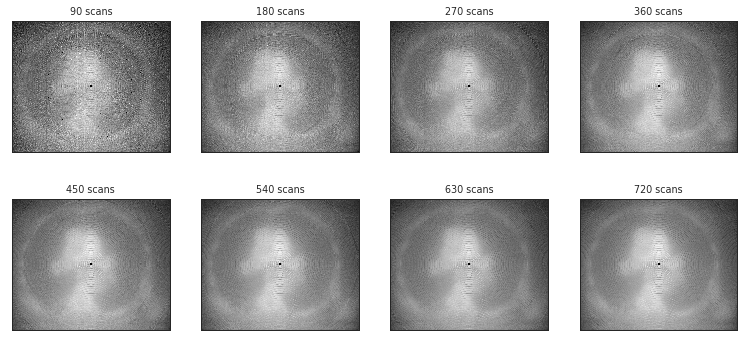
\includegraphics[width=\linewidth]{res/scans.png}
	\label{fig:scans}
	\caption{Zmiana liczby skanów}
\end{figure}

\begin{figure}[h]
	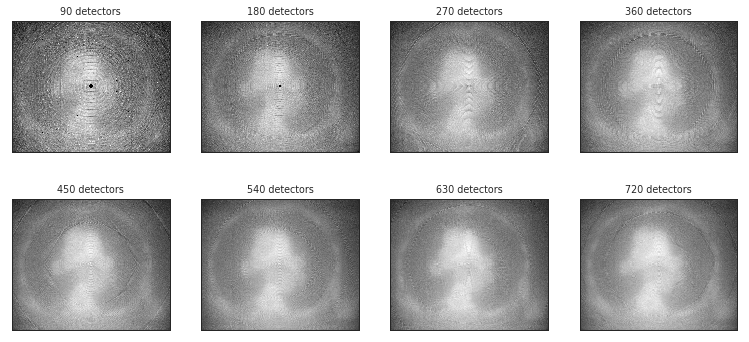
\includegraphics[width=\linewidth]{res/detec.png}
	\label{fig:detec}
	\caption{Zmiana liczby detektorów}
\end{figure}

\begin{figure}[h]
	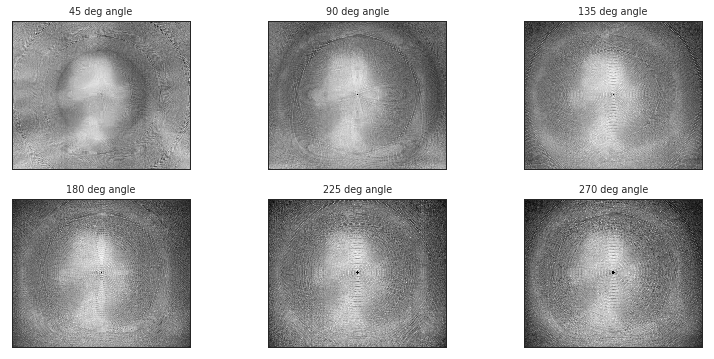
\includegraphics[width=\linewidth]{res/angle.png}
	\label{fig:angle}
	\caption{Zmiana rozwartości kąta}
\end{figure}

\end{document}

